\subsection{Race conditions}
\subsubsection{What is a race condition?}

A race condition occurs when two or more concurrent routines read and modify the same data simultaneously. When the shared data is not protected by synchronization tools, unpredictable errors can occur.

A simple data race can be demonstrated with the example below, when \code{foo()} and \code{bar()} are being executed concurrently:

\begin{minted}[linenos, bgcolor=LightGray]{c}
int x = 0;

void foo() {
  x += 1;
}

void bar() {
  x += 2;
}
\end{minted}

The race occurs because the increment operation is not atomic. In fact, an increment like \code{x += 1} consists of three separate steps:

\begin{enumerate}
  \item Reading the value of \code{x} from memory
  \item Adding 1 to the value of \code{x}
  \item Writing the result back to memory
\end{enumerate}

If \code{foo} and \code{bar} run concurrently, they may interleave their execution of these steps. That is, after \code{foo} has read the value of \code{x}, \code{bar} may also read \code{x} before \code{foo} has written the new value of \code{x} back to memory --- which produces an incorrect result. I've illustrated this principle on \autoref{fig:data-race}.

\begin{figure}[H]
  \centering
  \hbox{\makebox[\textwidth][c]{
    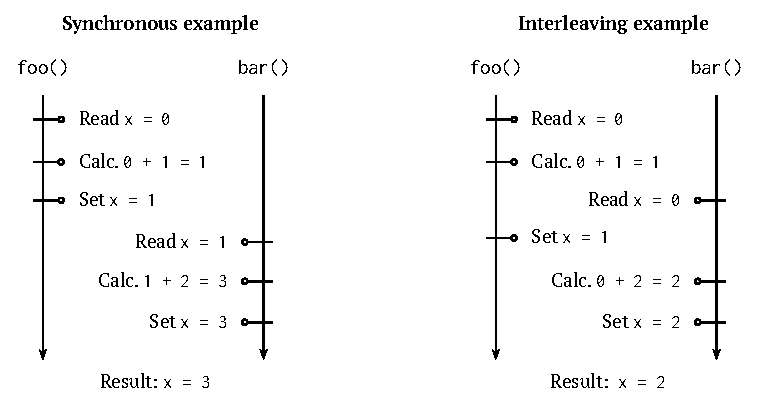
\includegraphics{figures/data-race-example.pdf}
  }}
  \caption{An illustration showing how \code{foo} and \code{bar} may be expected to run (left) versus how they can potentially interleave and produce incorrect results (right).}
  \label{fig:data-race}
\end{figure}

\subsubsection{Why race conditions are hard to debug}

The two cases illustrated in \autoref{fig:data-race} are far from the only outcomes. Data races can be very difficult to debug because the instructions can interleave in so many ways. And this is just with one increment and two concurrent routines. When you make the routines larger and increase the amount of them, it can be very, very difficult to find all possible outcomes.

On top of that, it can be difficult to reproduce a race condition because multithreaded programs are nondeterministic~\cite[p. 784]{computersystems}. This means that you cannot determine exactly how the program will run --- for example due to OS scheduling. Every time you run it, you may get a different outcome. If the race condition occurs very rarely, you may get a correct output most of the time and then only an incorrect output seemingly at random, making it hard to debug.

\subsubsection{Which instructions can you use to avoid race-conditions?}

In order to avoid race conditions, you can use synchronization primitives. In x86, you can use atomic CPU instructions, which are compositions of smaller ``sub-instructions'' (i.e. getting or setting a value), which are guaranteed to be executed atomically. Here, ``atomically'' means that while the instruction is executing, it has sole access to the shared data. Below, I have listed four atomic CPU instructions~\cite[slide 60]{concurrencyslides}:

\begin{enumerate}
  \item \textit{Fetch and add}, which increments some value with the given parameter. In x86, this is \code{LOCK INC}~\cite[p. 1170]{x86manual}.
  \item \textit{Compare and swap}, which compares a value $n$ in memory with a given parameter $v$. If $n$ and $v$ are equal, $n$ is overwritten with the value of another parameter $p$. In x86, this is \code{CMPXCHG}~\cite[p. 779]{x86manual}.
  \item \textit{Test and set}, which is used to set a value to 1 (true). A \textit{reset} would be the inverse operation, setting it to 0 (false). In x86, this is \code{LOCK BTS} (and \texttt{BTR} to reset)~\cite[p. 1170]{x86manual}.
  \item \textit{Memory barrier}, which prevents memory operation reordering. CPUs can optimize execution time by reordering instructions~\cite[slide 56-59]{concurrencyslides}, but this may cause issues in a concurrent environment (for example by reordering read/writes to memory). In x86, you can use \code{MFENCE} to use a memory barrier~\cite[p. 1170]{x86manual}.
\end{enumerate}

These instructions can be used to implement higher-level synchronization tools, such as a mutex. For example, you can create a loop that continuously attempts to set a lock flag with the test-and-set instruction. Alternatively you could use the compare-and-swap instruction to set a lock flag if it's 0. A naive mutex that uses a loop like this is called a spinlock~\cite[slide 64]{concurrencyslides}.

\subsubsection{Why are these instructions expensive?}

The core reason (pun intended) that atomic instructions are expensive is that each core must ensure exclusive access to the data it writes, and it needs to synchronize reads and writes with other cores, which takes time.

The Cache Coherence Problem describes the problem of synchronizing values across cores. CPUs use different layers of caches to improve performance, some of which are local to each core. This means that a shared value may have been cached by multiple cores. When a core updates this shared value, it needs to ensure that another core doesn't use the now stale version of that value. One strategy to do this is by making a cache invalidation request, which will cause all the other cores to get a cache miss the next time they access the value --- instead, they will have to fetch the updated value~\cite[slide 44-54]{concurrencyslides}.

However, atomicity is also needed when performing something like a cache invalidation request. Otherwise, multiple cores may try to invalidate each other's caches simultaneously. This can be achieved with bus locking~\cite[slide 55]{concurrencyslides}, which gives a core exclusive access to a specific bus (which could be main memory, an interconnect, or some other bus)~\cite[slide 55]{concurrencyslides}.

If shared data is often accessed and modified by multiple cores, atomic operations can be vulnerable to \textit{cache thrashing}: a (possibly severe) performance reduction caused by cores having excessively synchronize their caches.
